%************************************************
\chapter{Couche limite}\label{ch:couche}
%************************************************

\begin{figure}[ht]
	\centering
	\includegraphics[scale = 0.6]{./gfx/crop_vitesse=28_volume=003.png}
	\caption{Goutte d'eau de volume $0.03$ml}
\end{figure}
Notre goutte d'eau (de volume de l'ordre millilitre) est sur une paroi horizontale en présence d'un écoulement d'air.


Pour déterminer les vitesses de l'écoulement d'air au voisinage de notre goutte d'eau, nous devons nous intéresser à la couche limite parce que d'après la théorie sur la couche limite, l'écoulement d'un fluide en présence d'une paroi peut être séparé en deux régions dont l'une proche de la paroi où les effets visqueux ne peuvent être négligés par rapport aux effets inertiels et l'autre région à l'extérieur de la précédente (avec une frontière commune) où les effets visqueux peuvent être négligés.

La couche limite est cette région proche de la paroi où les effets visqueux ne peuvent être négligés.

C'est Prandtl qui fut le premier à définir la couche limite. 

\section{Équations de la couche limite }

Les équations de la couche limite sont définies pour un écoulement bidimensionnel et nous nous les donnerons uniquement pour le cas d'un écoulement laminaire puisque nos écoulements étaient laminaires dans nos expériences.

Soit $u$ la vitesse de l'écoulement parallèle à la paroi suivant l'axe $x$ et $v$ la vitesse normale à la paroi suivant l'axe $y$.

Soit $U$ et $V$ les vitesses caractéristiques dans la couche limite respectivement de $u$ et $v$ ($\left| u \right| \sim U$ et $\left| v \right| \sim U$).

Soit $L$ et $\delta$ la taille caractéristique de la couche limite suivant respectivement l'axe $x$ et l'axe $y$ ($\left| x \right| \sim L$ et $\left| y \right| \sim \delta$).

En plus de l'hypothèse d'écoulement bidimensionnel, les hypothèses faites sont : la pesanteur est négligée, l'écoulement est stationnaire, incompressible, $\frac{\delta}{L} << 1$ et les effets visqueux et inertiels sont du même ordre de grandeur dans la couche limite.


De l'équation de Navier-Stokes et de continuité, on trouve pour équations de la couche limite:

\begin{align}	
	\frac{\partial u}{\partial x} 
	+
	\frac{\partial v}{\partial y} 
	&= 0 \\
	u\frac{\partial u}{\partial x} + 
	v\frac{\partial u}{\partial y} 
	&= - \frac{1}{\rho}
	\frac{\partial p}{\partial  x} +
	\nu
	\frac{\partial^{2} u}{\partial  y^{2}} \\
	\frac{\partial p}{\partial y} 
	&= 0
\end{align}
\section{Équations de Blasius}
L'équation de Blasius est l'équation de la couche limite pour un écoulement laminaire sur une plaque plane dont la vitesse $U$ loin de la couche limite est constante et parallèle à l'axe $x$.

Soit $\varphi$ la fonction de courant tel que :

\begin{align*}
	u(x,y) &= 
	\frac{\partial \varphi}{\partial y} \\
	v(x,y) &= - 
	\frac{\partial \varphi}{\partial x}
\end{align*}

On pose :

\begin{align*}
	\eta &= y \sqrt{\frac{U}{2\nu x }} \\
	\varphi &= \sqrt{2\nu U x} f(\eta)
\end{align*}


On trouve ainsi l'équation de la couche limite de Blasius à partir des équations de la couche limite :
\begin{equation}	
	\frac{d^{3}f}{d\eta^{3}} + f\frac{d^{2} f}{d\eta^{2}} = 0
\end{equation}
Avec les conditions aux limites:
\begin{align}
	u(x,0) &= 0 &\Rightarrow &&
	\left.
	\frac{d f}{d \eta}     \right|_{\eta = 0} &= 0
	\\
	v(x,0) &= 0 &\Rightarrow &&
	f(0) &= 0
	\\
	u(x,\infty) &= U &\Rightarrow &&
	\left.
	\frac{d f}{d \eta} \right|_{\eta = \infty} &= 1
\end{align}
\newpage
\begin{figure}[ht]
	\centering
	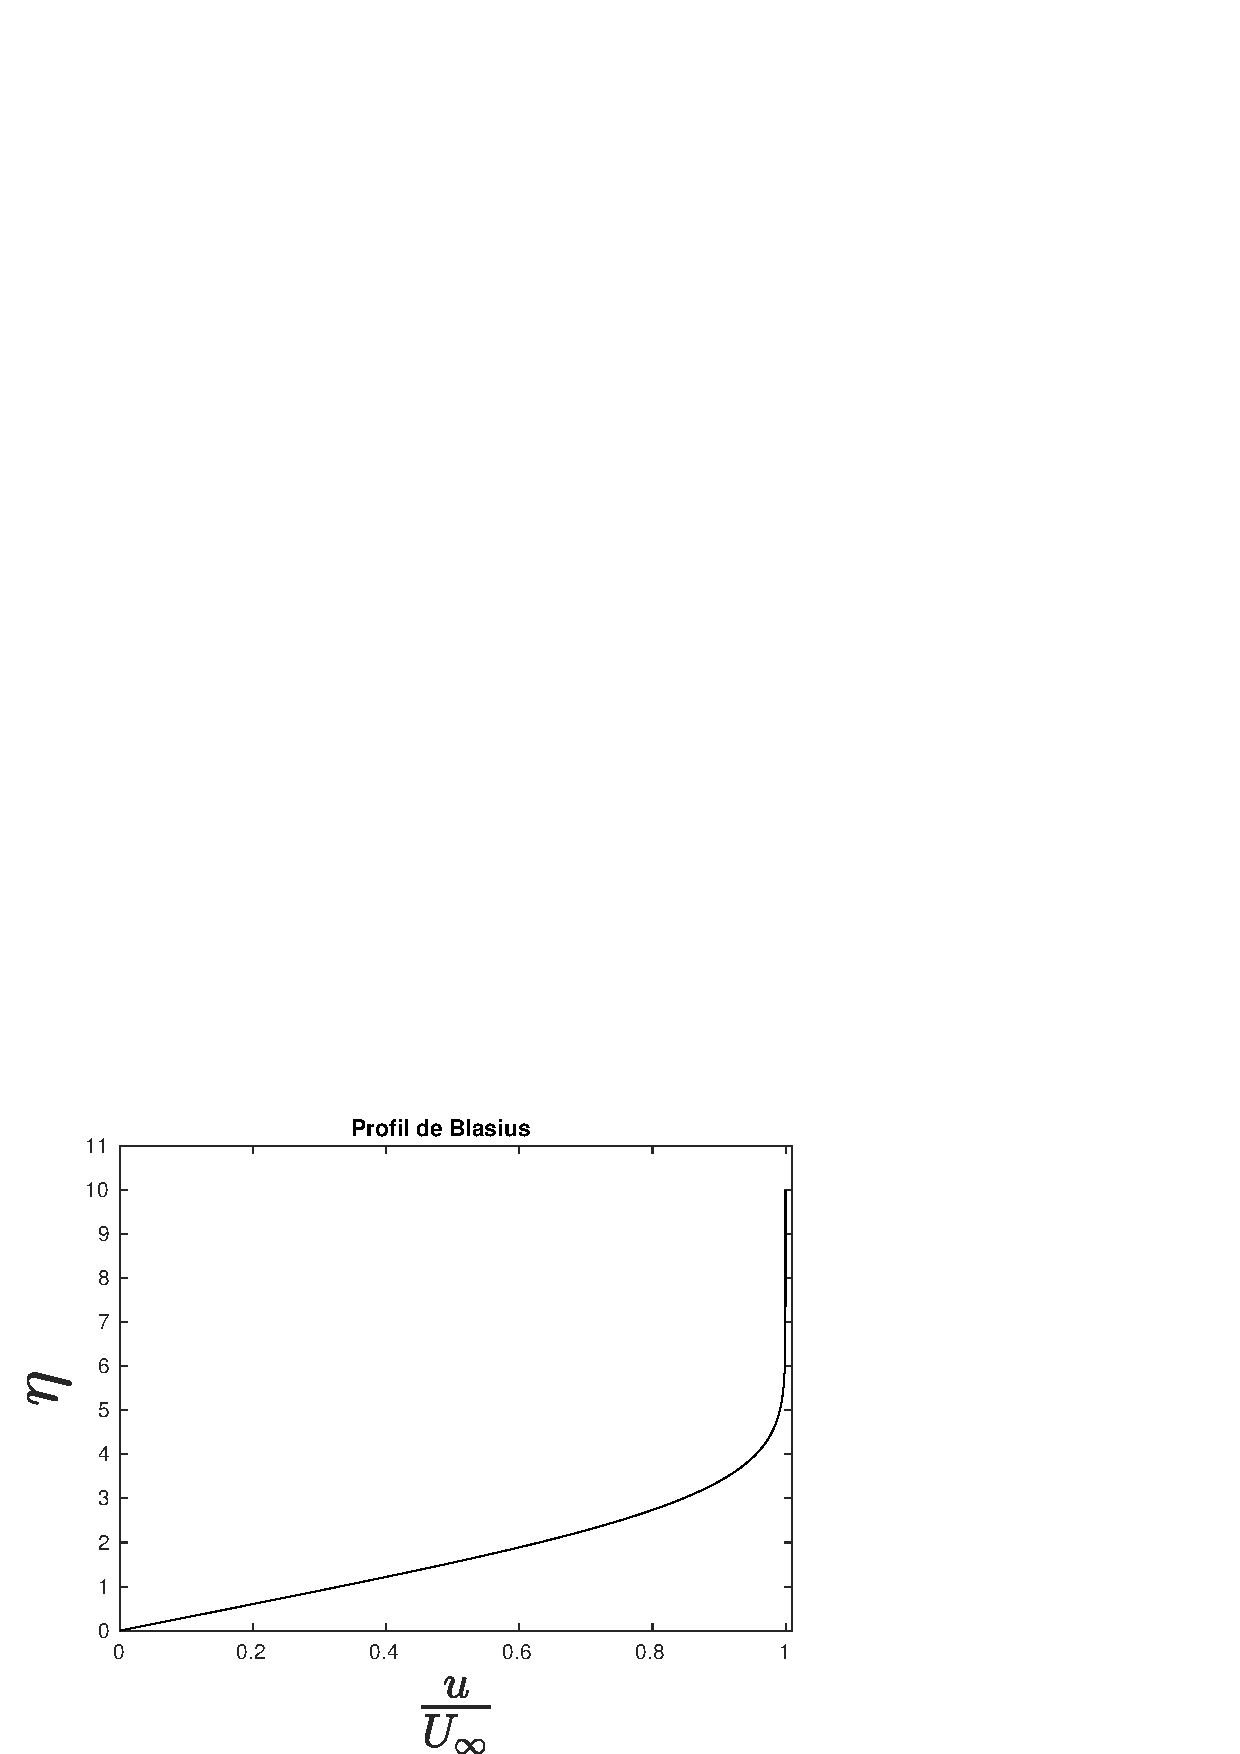
\includegraphics[scale = 0.6]{./gfx/Blasius.png}
	\caption{Profil de Blasius}
\end{figure}
Les grandeurs que nous avons comparées expérimentalement provenant du résultat des équations de Blasius sont l'épaisseur de déplacement $\delta_{1}$, l'épaisseur de quantité de mouvement $\delta_{2}$ et le coefficient de frottement $C_{f}$
\section{Épaisseur de déplacement}
L'épaisseur de déplacement $\delta_{1}$ à $x$ fixé est définie par:
\begin{equation}
	\delta_{1} = 
	\int_{0}^{^\infty}
	\left(
	1 - 
	\frac{u}{U}
	\right)
	dy
	\approx \frac{1.72x}{\sqrt{Re_{x}}}
\end{equation}
\section{Épaisseur de quantité de mouvement}
L'épaisseur de quantité de mouvement $\delta_{2}$ à $x$ fixé est définie par:
\begin{equation}
	\delta_{2} = 
	\int_{0}^{^\infty}
	\frac{u}{U}
	\left(
	1 - 
	\frac{u}{U}
	\right)
	dy
	\approx \frac{0.664x}{\sqrt{Re_{x}}}
\end{equation}
\section{Coefficient de frottement à la paroi}
Le coefficient de frottement à la paroi $C_{f}$ à $x$ fixé est défini par:
\begin{equation}
	C_{f} =
	\frac{2\tau_{y=0}}{\rho U^{2}} =
	\frac{2\nu}{U^{2}}
	\left.
	\frac{\partial u}{\partial y}
	\right|_{y = 0} \approx \frac{0.664}{\sqrt{Re_{x}}}
\end{equation}
\section{Comparaisons avec nos expériences}
Nous avons effectué nos mesures à l'aide de l'anémomètre à fil chaud et nous trouvons avec :
\begin{align*}
	x &= 0.55m\\
	Re_{x} &= \frac{Ux}{\nu}\\
	\nu &= 1.5e-5 m^{2}.s^{-1}~~\text{à}~~T = 25^{o}C; 
\end{align*}
\begin{table}[ht]
	\centering
	\begin{tabular}{cc}
		\hline\\
		$U(m/s)$ & Reynolds\\
		\hline
   15 & 550000.00\\
   20 & 733333.33\\
   24 & 880000.00\\
   28 & 1026666.7
	\end{tabular}
	\caption{Nombre de Reynolds $Re_{x}$}
\end{table}
\begin{table}[ht]
	\centering
	\begin{tabular}{cccc}
		\hline\\
		$U(m/s)$ & $\delta_{1Blasius}(mm)$ &
		$ \delta_{1Experience}(mm)$ & 
		 erreur relative\\
		\hline
		15   & 1.27   & 1.24   & 2.69\%\\
		20   & 1.11   & 1.10   & 0.61\%\\
		24   & 1.02   & 0.99   & 3.13\%\\
		28   & 0.96   & 0.95   & 1.55\%
	\end{tabular}
	\caption{Comparaison épaisseur de déplacement $\delta_{1}$}
\end{table}
\begin{table}[ht]
	\centering
	\begin{tabular}{cccc}
		\hline\\
		$U(m/s)$ & $\delta_{2Blasius}(mm)$ &
		$ \delta_{2Experience}(mm)$ & 
		 erreur relative\\
		\hline
   15 & 0.49   & 0.47   & 3.64\%\\
   20 & 0.43   & 0.41   & 4.62\%\\
   24 & 0.40   & 0.37   & 6.08\%\\
   28 & 0.37   & 0.35   & 6.92\%
	\end{tabular}
	\caption{Comparaison épaisseur de quantité de mouvement $\delta_{2}$}
\end{table}
\begin{table}[ht]
	\centering
	\begin{tabular}{cccc}
		\hline\\
		$U(m/s)$ & $C_{fBlasius}$ &
		$ C_{fExperience}$ & 
		 erreur relative\\
		\hline
   15 & 8.92e-04   & 9.19e-04   & 2.89\%\\
   20 & 7.77e-04   & 7.67e-04   & 1.31\%\\
   24 & 7.20e-04   & 7.33e-04   & 1.85\%\\
   28 & 6.75e-04   & 6.67e-04   & 1.26\%
	\end{tabular}
	\caption{Comparaison coefficient de frottement $C_{f}$}
\end{table}
\begin{figure}[ht]
	\centering
	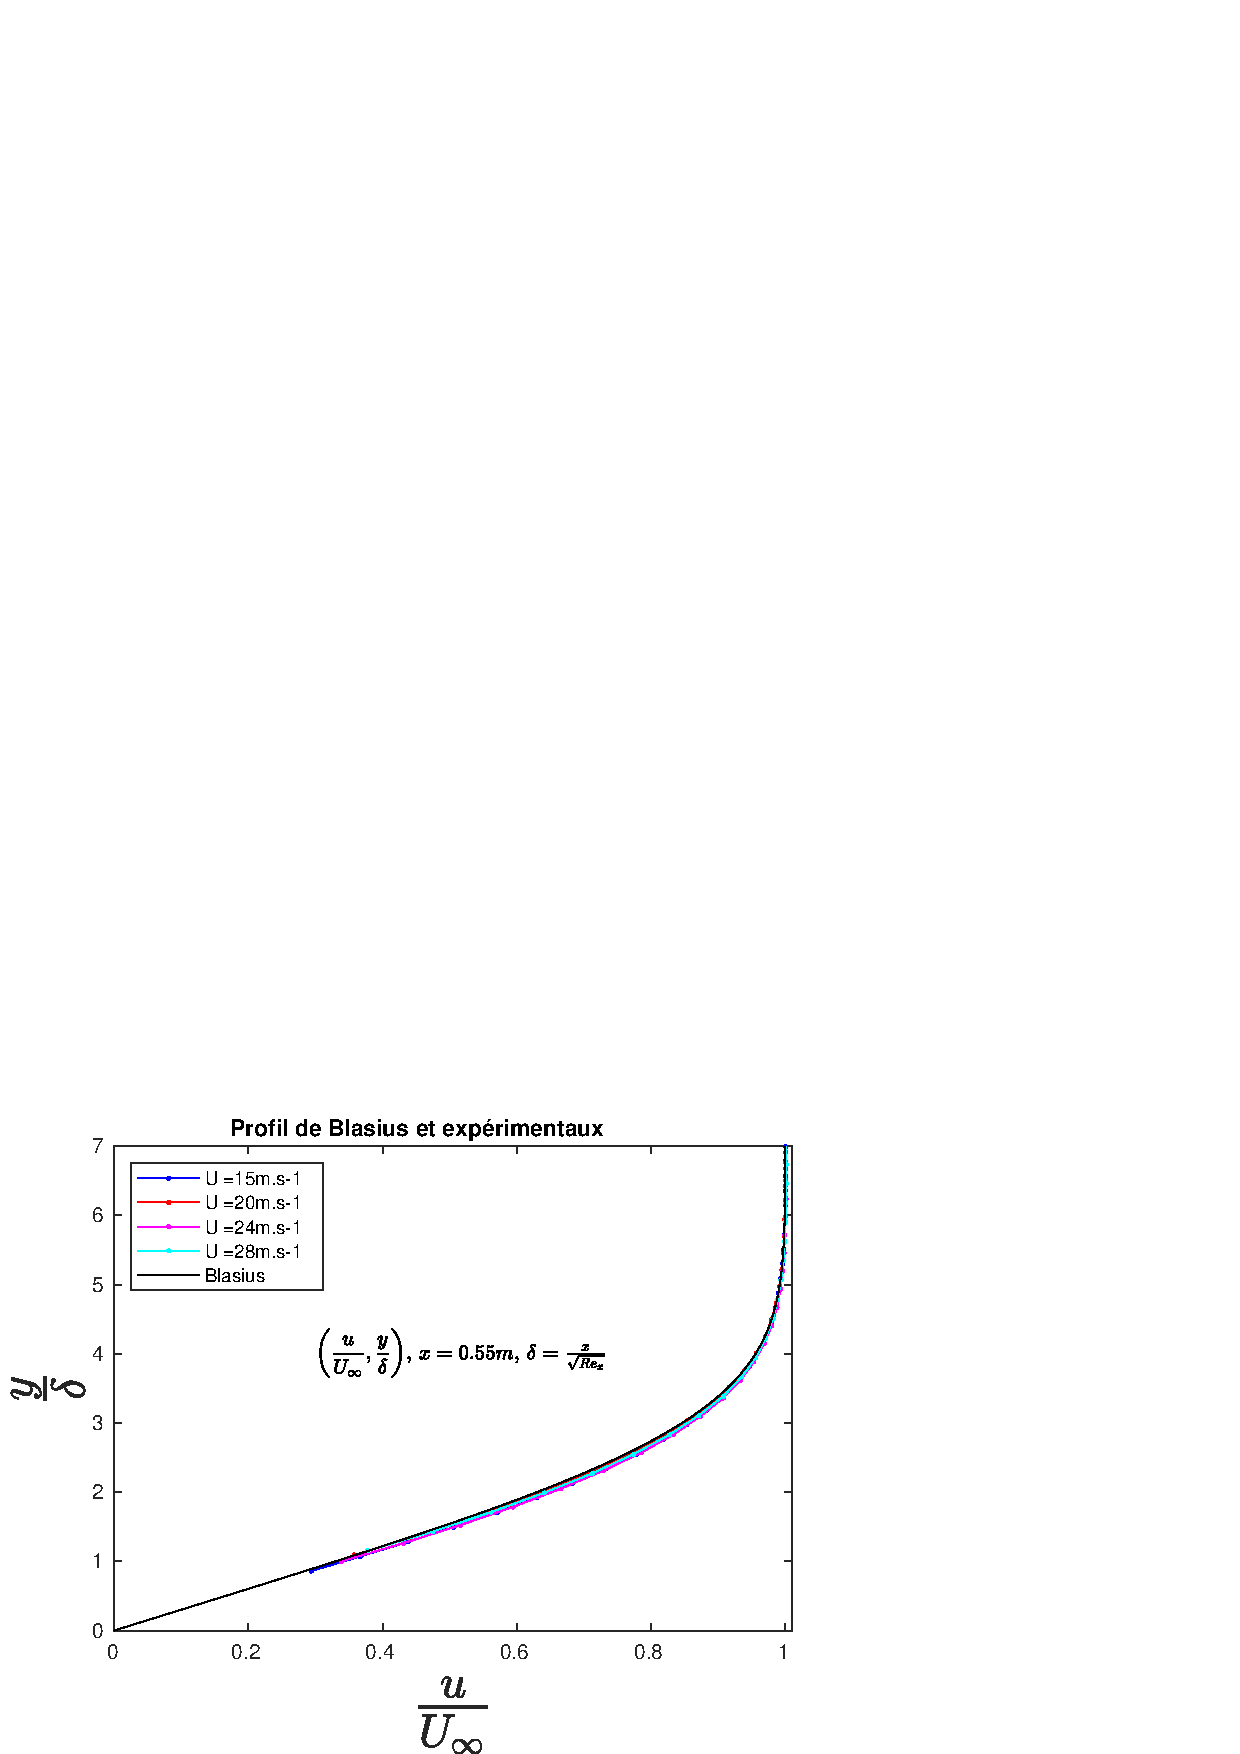
\includegraphics[scale = 0.6]{./gfx/Bla.png}
	\caption{Profil de Blasius et expérimentaux}
\end{figure}
\newpage
Nous avons pu constater que l'épaisseur de la couche limite, l'épaisseur de la quantité de mouvement, le coefficient de frottement à la paroi et nos profils de vitesses sont tous très proches de leur équivalent dans la théorie de la couche limite de Blasius.
%\begin{thebibliography}{}
%\bibitem{RefJ}
%% Format for Journal Reference
%Author, Article title, Journal, Volume, page numbers (year)
%% Format for books
%\bibitem{RefB}
%Author, Book title, page numbers. Publisher, place (year)
%\end{thebibliography}
